\section{Verification challenge and main ideas}
\label{sc:overview}

%%\begin{wrapfigure}[9]{r}[0pt]{0.4\textwidth} 
%% \begin{figure}
%% %
%% \centering
%% \begin{tabular}{l l l}
%% %
%% %  
%% \begin{minipage}[l]{.30\textwidth}
%% \begin{alltt}
%% \num{1}  write (p, v): () \{
%% \num{2}    \act{write} (p, v);
%% \num{3}    b <- \act{read} (S);
%% \num{4}    \textbf{if} b 
%% \num{5}    \textbfthen \act{transfer} (p, v);
%% \num{6}    \textbf{else skip};\}
%% \end{alltt} 
%% \end{minipage}
%% %
%% & \hfill
%% %
%% \begin{minipage}[l]{.6\textwidth}
%% \begin{alltt}
%% \num{1}  scan (): \(A {\times} A\)  \{
%% \num{2}    \act{write} (S, true);
%% \num{3}    \act{write} (fx,\( \bot\));
%% \num{4}    \act{write} (fy,\( \bot\));
%% \num{5}    vx <- \act{read} (x);
%% \num{6}    vy <- \act{read} (y);
%% \num{7}    \act{write}(S, false);
%% \num{8}    ox <- \act{read} (fx);
%% \num{9}    oy <- \act{read} (fy);
%% \num{10}   \textbf{let} rx = \textbf{if} ox \(\neq \bot\) \textbfthen ox \textbf{else} vx;  
%% \num{11}   \textbf{let} ry = \textbf{if} oy \(\neq \bot\) \textbfthen oy \textbf{else} vy;  
%% \num{11}   \act{relink}(rx, ry);
%% \num{12}   \textbf{return} (rx, ry);
%% \end{alltt} 
%% \end{minipage}
%% %
%% \end{tabular}
%% %
%% \caption{Jayanti's single-scanner, single-writer snapshot algorithm}
%% \label{fig:jayanti}
%% \end{figure}
%\end{wrapfigure}

\newcommand{\actwrite}[2]{{#1}\,{:=}\,{#2}}

% The following version saves a little more space
\begin{figure}
%
\centering
\begin{tabular}{c@{\ \ \ \ \ }c}
%  
\begin{minipage}[t][3.7cm][t]{.5\textwidth}
\small
\begin{alltt}
\num{1} write (p : ptr, v : \(A\)) \{
\num{2}  \actwrite{p}{v};
\num{3}  b \tbnd \act{read}(S);
\num{4}  if b 
\num{5}  then \actwrite{(f_of p)}{v}
\num{6}  {else return} \}

  f_of (p : ptr) \{
   return p = x ? fx : fy \}
\end{alltt}
\end{minipage}
%
&
\begin{minipage}[t][3.7cm][t]{.5\textwidth}
\small
\begin{alltt}
\num{ 7} scan (): \(A {\times} A\)  \{
\num{ 8}  \actwrite{S}{true};
\num{ 9}  \actwrite{fx}{\(\bot\)}; \actwrite{fy}{\(\bot\)};
\num{10}  vx \tbnd \act{read}(x); vy \tbnd \act{read}(y);
\num{11}  \actwrite{S}{false};
\num{12}  ox \tbnd \act{read}(fx); oy \tbnd \act{read}(fy);
\num{13}  rx \tbnd if (ox \(\neq\bot\)) then ox {else} vx;  
\num{14}  ry \tbnd if (oy \(\neq\bot\)) then oy {else} vy;  
\num{15}  return (rx, ry) \}
\end{alltt} 
\end{minipage}
%
\end{tabular}
%
\caption{Jayanti's single-scanner/single-writer snapshot algorithm.}
\label{fig:jayanti-snapshot}
\end{figure}



%\newcommand{\fx}{\mathtt{fx}}
%\newcommand{\fy}{\mathtt{fy}}
%\newcommand{\x}{\mathtt{x}}
%\newcommand{\y}{\mathtt{y}}
%\newcommand{\s}{\mathtt{S}}

\newcommand{\fx}{fx}
\newcommand{\fy}{fy}
\newcommand{\x}{x}
\newcommand{\y}{y}
\newcommand{\s}{S}

Jayanti's snapshot algorithm~\cite{Jayanti:STOC05} provides the
functionality of a shared array of size $m$, operated on by two
procedures: {\tt write}, which stores a given value into an element,
and {\tt scan}, which returns the array's contents. We use the
\emph{single-writer}/\emph{single-scanner} version of the algorithm,
which assumes that at most one thread writes into an element, and at
most one thread invokes the scanner, at any given time.
% 
%where a thread acquires a writer lock for a particular element before
%writing into it, and a scanner before scanning. A scanner lock does
%not preclude writing, and a writer lock for an element does not
%preclude scanning, or writing into other elements. 
This is the simplest of Jayanti's algorithms, but it already exhibits
linearization points of dynamic nature. We also
restrict the array size to $m=2$ (i.e., we consider two pointers $\x$
and $\y$, instead of an array). This removes some tedium from
verification, but exhibits the same conceptual challenges.
 
The difficulty in this snapshot algorithm is ensuring that the scanner
returns sound values of $\x$ and $\y$. A naive scanner, which simply
reads $\x$ and $\y$ in succession, is unsound. To see why, consider
the following scenario, starting with $\x=5$, $\y=0$. The scanner
reads $\x$, but before it reads $\y$, another thread preempts it, and
changes $\x$ to $2$ and $\y$ to $1$. The scanner continues to read
$\y$, and returns $\x=5, \y=1$, but this was never the contents of the
memory.

To ensure a sound snapshot, Jayanti's algorithm internally keeps
additional \emph{forwarding pointers} $\fx$ and $\fy$, and a boolean
\emph{scanner bit} $\s$. The implementation is given in
Figure~\ref{fig:jayanti-snapshot}, and \emph{assumes} the
single-writer/single-scanner setup (the assumption can be enforced
with wrapper locking code, which we omit here for simplicity, but
consider in our Coq proofs).
%
The intuition is as follows. A writer storing $v$ into $p$ (line~2),
will additionally store $v$ into the forwarding pointer for $p$
(line~5). If the scanner missed the write and instead read the old
value of $p$ (line~10), it will have a chance to catch $v$ via the
forwarding pointer (line~12). The scanner bit $S$ is used by writers
(line~3) to detect a scan in progress, and forward $v$.

{
\setlength{\belowcaptionskip}{-5pt} 
\begin{figure}[t]
%
\centering  
\begin{subfigure}[t]{1\textwidth}
\centering
\small  
\begin{tabular}{l || l || l}
  \texttt{l: }\texttt{write (x,2);} &
   \multirow{2}{*}{\texttt{c: scan ()}} & 
    \multirow{2}{*}{\texttt{r: write (x,3)}}  \\
  \phantom{\texttt{l: }}\texttt{write (y,1)} & &   
\end{tabular}
\caption{\label{fig:weird:code}}
\end{subfigure}
\begin{subfigure}[b]{1\textwidth}
\begin{tabular}{l@{\hfill} l@{\hfil} l}
\begin{minipage}[t][3cm][t]{0.33\textwidth}
\small
\begin{alltt}
\num{1}  c: \actwrite{S}{true}
\num{2}  c: \actwrite{fx}{\(\bot\)}
\num{3}  c: \actwrite{fy}{\(\bot\)}
\num{4}  c: \act{read}(x)  // vx <- 5
\num{5}  c: \act{read}(y)  // vy <- 0
\num{6}  l: \actwrite{x}{2}
\num{7}  l: \act{read}(S)  // b <- true
\end{alltt}
%% \begin{alltt}
%% \num{1}  c: scan () 
%% \num{2}  c: \act{write}(S, true)
%% \num{3}  c: \act{write}(fx,\( \bot\))
%% \num{4}  c: \act{write}(fy,\( \bot\))
%% \num{5}  c: \act{read}(x)      // vy <- 5
%% \num{6}  c: \act{read}(y)      // vx <- 0
%% \num{7}  l: write (x, 2)
%% \num{8}  l: \act{write}(x, 2)
%% \num{9}  l: \act{read}(S)      // b <- true
%% \num{10} l: \act{write}(fx, 2) 
%% \num{11} l: ret ()
%% \num{12} r: write (x, 3)
%% \end{alltt}
%% \gad{will clean up after final version set}
\end{minipage}
&
\begin{minipage}[t][3cm][t]{0.33\textwidth}
\small
\begin{alltt}
\num{8}  l: \actwrite{fx}{2} 
\num{9}  l: ret ()
\num{10} r: \actwrite{x}{3}
\num{11} l: \actwrite{y}{1}
\num{12} l: \act{read}(S)  // b <- true
\num{13} l: \actwrite{fy}{1}
\num{14} l: ret ()
\end{alltt}
\end{minipage}
&
\begin{minipage}[t][3cm][t]{0.33\textwidth}
\small
\begin{alltt}
\num{15} c: \actwrite{S}{false}
\num{16} r: \act{read}(S)  // b <- false
\num{18} r: ret ()
\num{18} c: \act{read}(fx) // ox <- 2
\num{19} c: \act{read}(fy) // oy <- 1
\num{20} c: ret (2,1)
\end{alltt} 
%% \begin{alltt}
%% \num{13} r: \act{write}(x, 3)
%% \num{14} l: write (y, 1)
%% \num{15} l: \act{write}(y, 1)
%% \num{16} l: \act{read}(S)      // b <- true
%% \num{17} l: \act{write}(fy, 1)
%% \num{18} l: ret ()
%% \num{19} c: \act{write}(S, false)
%% \num{20} r: \act{read}(S)      // b <- false
%% \num{21} r: ret ()
%% \num{22} c: \act{read}(fx)     // ox <- 2
%% \num{23} c: \act{read}(fy)     // oy <- 1
%% \num{24} c: ret (2,1)
%% \end{alltt} 
\end{minipage}
%
\end{tabular}
\caption{\label{fig:weird:exec} A possible interleaving of the threads
  in~(\subref{fig:weird:code}).}
\end{subfigure}
%
\caption{\label{fig:weird} An example leading to a scanner miss.}
\end{figure}
}

% \gad{Remember that \small should go inside minifigures!}

 
As Jayanti proves, this implementation is linearizable. Informally,
every overlapping calls to {\tt write} and {\tt scan} can be
rearranged to appear as if they occurred sequentially.  To illustrate,
consider the program in Figure~\ref{fig:weird:code}, and one possible
interleaving of its primitive memory operations in
Figure~\ref{fig:weird:exec}. The threads {\tt l}, {\tt c}, and {\tt
  r}, start with $\x = 5, \y = 0$.
%
The thread {\tt c} is scheduled first, and through lines~2-6 sets the
scanner bit, clears the forwarding pointers, and reads $\x = 5, \y =
0$. Then {\tt l} intervenes, and in lines~7-11, overwrites $\x$ with
$2$, and seeing $\s$ being set, forwards $2$ to $\fx$. Next, {\tt r}
and {\tt l} overlap, writing $3$ into $\x$ and $1$ into $\y$. However,
while $1$ gets forwarded to $\fy$ (line 13), $3$ is not forwarded to
$\fx$, because $\s$ was turned off in line 15. Thus, when {\tt c}
reads the forwarded values (lines 18, 19), it returns $\x = 2, \y =
1$. 

While $\x\,{=}\,2, \y\,{=}\,1$ was never the contents of the memory,
returning this snapshot is nevertheless justified because we can
\emph{pretend} that the scanner \emph{missed} {\tt r}'s write of
$3$. Specifically, the events in Figure~\ref{fig:weird:exec} can be
\emph{reordered} to represent the following sequential execution.
%
\begin{equation}
\mathtt{write\, (x, 2);\ write\, (y,1);\ scan\, ();\ write\, (x,
  3)} \label{eq:lin}
\end{equation}
The client programs cannot discover that a different scheduling
actually took place in real time, because they can access the internal
state of the algorithm only via {\tt write} and {\tt scan}.

This kind of temporal reordering is the most characteristic aspect of
linearizability proofs, which typically describe the reordering by
listing the linearization points of each procedure. At a linearization
point, the procedure's operations can be spliced into the execution
history as an uninterrupted chunk. For example, in Jayanti's proof,
the linearization point of {\tt scan} is at line~11
(Figure~\ref{fig:jayanti-snapshot}), where the scanner bit is
unset. The linearization point of {\tt write}, however, may vary. If
{\tt write} starts before an overlapping {\tt scan}'s line 11, and
moreover, the {\tt scan} misses the {\tt write} (note the dynamic
nature of this property), then {\tt write} should appear after {\tt
  scan}; that is, the {\tt write}'s linearization point is right after
{\tt scan}'s linearization point at line~11. 
%
Otherwise, {\tt write}'s linearization point is at line~2.
%
In the former case, {\tt write} has a \emph{future-dependent},
\emph{non-local}, \emph{non-regional} linearization point, as we can
only identify it in the execution of {\tt scan} in a different thread,
and only \emph{after} the execution of {\tt write} has terminated. For
instance, in Figure~\ref{fig:weird:exec} the execution of the second
{\tt write} in \texttt{l} terminates at step 14, yet the decision of
its position in the linearization order is taken only when the scanner
is at step 15.


\begin{figure}[t]
%\captionsetup[subfigure]{justification=centering}
\begin{subfigure}[t]{0.49\textwidth}
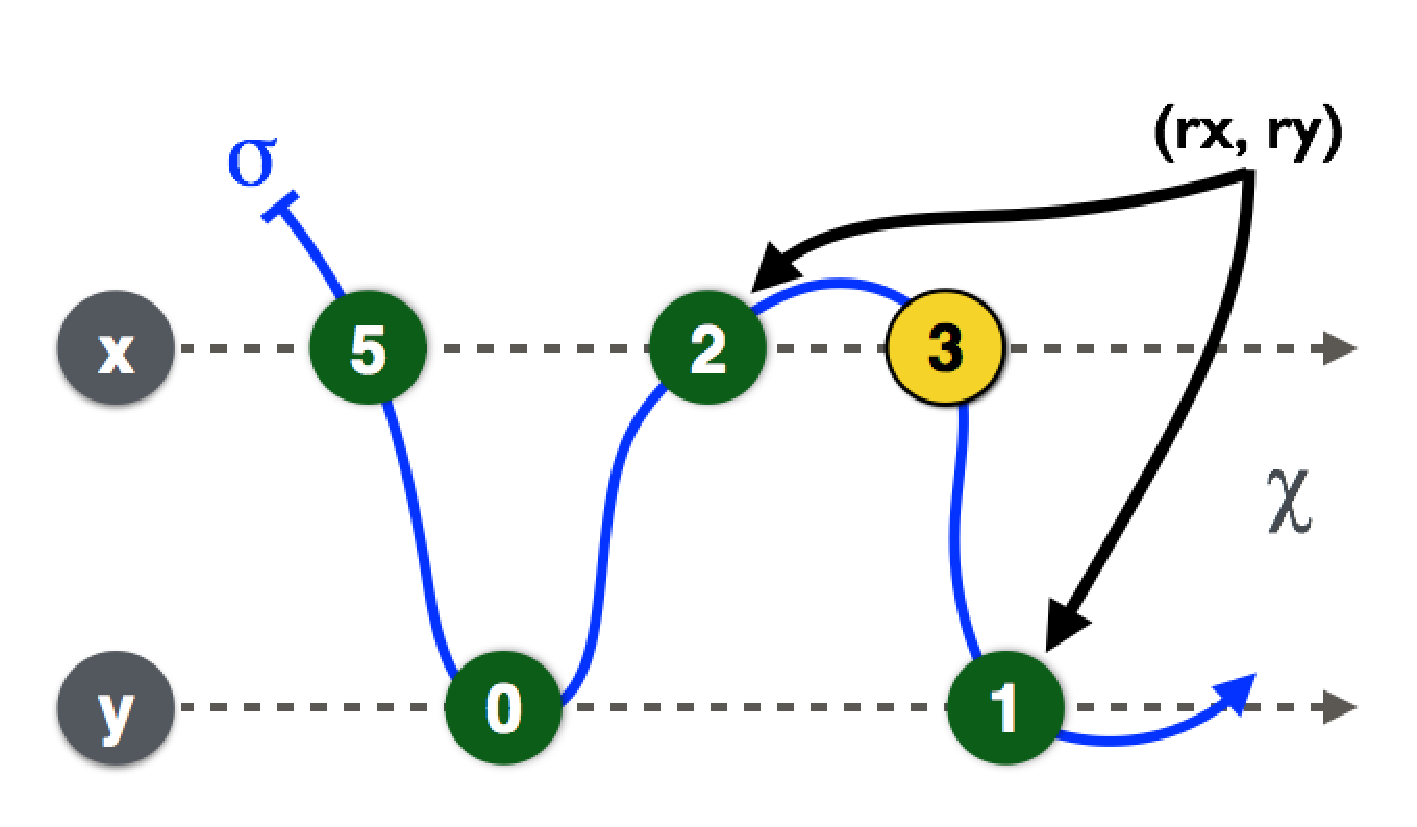
\includegraphics[width=6.1cm]{relink-before3.pdf}
\caption{\label{fig:reorder:before}} % Logical $=$ Real Time order, not a snapshot}
\end{subfigure} \hfill
\begin{subfigure}[t]{0.49\textwidth}
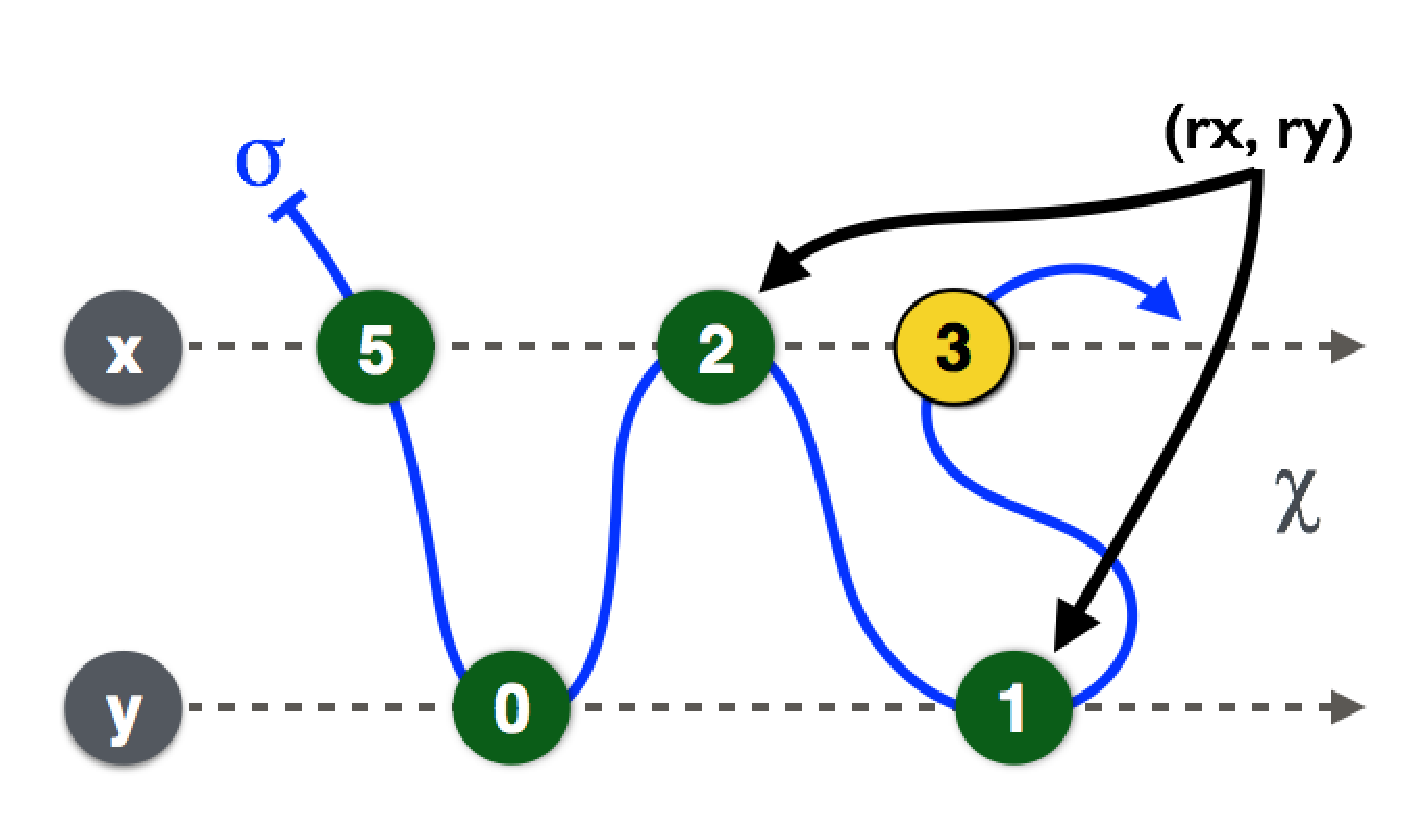
\includegraphics[width=6.1cm]{relink-after3.pdf}
\caption{\label{fig:reorder:after}} % Logical $\neq$ Real Time order, snapshot OK}
\end{subfigure}%
%
\caption{\label{fig:reorder} Changing the logical ordering (solid line
  $\ordlist$) of write events from (5, 0, 2, 3, 1) in
  (\subref{fig:reorder:before}) to (5, 0, 2, 1, 3) in
  (\subref{fig:reorder:after}), to reconcile with {\tt scan} returning
  the snapshot $\x=2, \y=1$, upon missing the write of $3$. Dashed
  lines $\hist$ represent real-time ordering.}
\end{figure}


Obviously, the high-level pattern of the proof requires tracking a
logical ordering of the {\tt write} and {\tt scan} events, which
differs from the real time. As the logical ordering is inherently
dynamic, depending on properties such as {\tt scan} missing a {\tt
  write}, we formalize it in Hoare logic, by keeping it as a list of
events in auxiliary state that can be dynamically reordered as
needed. For example, Figure~\ref{fig:reorder:before} shows the
situation in the execution of {\tt scan} that we reviewed above, where
the logical ordering coincides with real-time ordering, but is unsound
for the snapshot $\x=2, \y=1$ that {\tt scan} wants to return. In that
case, the auxiliary code with which we annotate {\tt scan},
will change the list in-place, as shown in
Figure~\ref{fig:reorder:after}.

Our challenge then lies in reconciling the following two conflicting
requirements. First, we need to implement the reordering discipline so
that the subsequent calls to {\tt write} and {\tt scan} preserve the
established logical order of the past events. This will be
accomplished by introducing yet further structures into the auxiliary
state and code. Second, we have to engineer Hoare triples for {\tt
  write} and {\tt scan} to be \emph{intuitive} and \emph{usable} by
clients, but also to \emph{not expose} the specifics of the reordering
discipline, which is internal to the snapshot object. 
%We discuss these issues next.



